\section{Fluxo do Jogo}
Este capítulo tem por objetivo descrever e mostrar a maneira como os diversos elementos que compõe o jogo interligam-se entre si.

\subsection{Progressão do Jogo}
Para a correta representação dos elementos que compõe o jogo um diagrama de máquinas de estados foi utilizado, o qual podem ser visualizado por meio da figura \ref{img:fluxo_jogo}.

\begin{figure}[!ht]
 \centering
 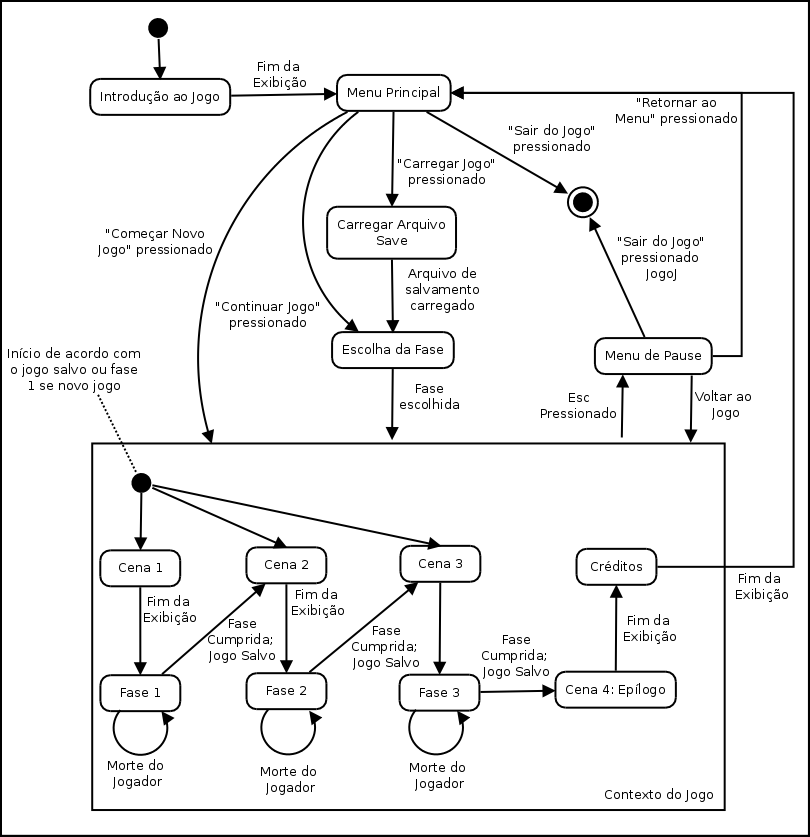
\includegraphics[scale=0.40]{fluxo_jogo.png}
 \caption{Diagrama do Fluxo do Jogo}
 \label{img:fluxo_jogo}
\end{figure}

Ao iniciar o aplicativo, o jogo tem início com a introdução e, logo após, passa o controle da interação ao menu principal. Neste menu, são previstas 4 opções: ``Começar um Novo Jogo'', ``Carregar Jogo'', ``Continuar Jogo'' e ``Sair''. ``Sair'' leva o personagem ao estado final do diagrama de máquina de estados, encerrando assim o aplicativo. ``Carregar Jogo'' permite ao jogador escolher um jogo salvo e passa, logo após, o controle à escolha das fases disponíveis no perfil carregado. ``Continuar jogo permite ao jogador continuar a campanha do último perfil jogado. ``Começar um Novo Jogo'' inicia uma nova campanha, onde o jogador é levado a assistir a cena 1, pela qual o enredo é apresentado. Após finalização desta, tem início à primeira fase. Com o decorrer do jogo,  diversas cenas e fases são alcançadas no caso de sucesso do usuário ao  cumprir os objetivos estabelecidos. Com a devida concretização da terceira fase, o epílogo e os créditos são apresentados, os quais devolvem, após finalizados, a interação ao controle do menu principal. Durante o jogo, com a eventual morte do personagem principal, o mesmo é levado ao último \textit{checkpoint} registrado. No caso da tecla Esc ser pressionada, a interação é pausada e, neste ponto, é possível retornar ao jogo, voltar ao menu principal ou sair para o ambiente de trabalho, finalizando assim o aplicativo.

No que diz respeito aos elementos contidos no fluxo do jogo representado pelo diagrama, os mesmos são elicitados e discutidos abaixo:
\begin{itemize}
\item \textit{Introdução ao Jogo:} a introdução é responsável por apresentar ao usuário informações referentes ao jogo em si, tais como a plataforma utilizada, os integrantes da equipe de trabalho, a disciplina e o professor;
\item \textit{Menu Principal:} o menu principal é o local onde são agrupados comandos que fornecem o ponto de partida ao jogo, com ações tais como "Começar um Novo Jogo" e "Carregar Jogo". É também o local onde o jogador é levado logo após a introdução inicial descrita acima;
\item \textit{Começar Novo Jogo:} opção do menu principal cujo acionamento leva o jogador à primeira etapa do contexto do jogo, o tutorial de aprendizado inicial. Ao escolher esta opção, o jogo se inicia;
\item \textit{Carregar Jogo:} opção do menu principal cujo acionamento possibilita ao jogador a escolher um jogo salvo. Esta opção permite ao jogador continuar uma ação interrompida em interações passadas;
\item \texteit{Continuar Jogo:} opção do menu principal cujo acionamento possibilita ao jogador continuar o jogo do último perfil utilizado;
\item \textit{Escolher Fase:} etapa de escolha de fase desejada, a qual torna-se disponível após a escolha do jogo salvo. Por meio dela é possível escolher dentre as fases já completadas que estiverem contidas dentro de um arquivo de jogo salvo;
\item \textit{Sair do Jogo:} opção presente tanto no menu principal, quanto no secundário, de \textit{pause}, a qual, em caso de acionamento, leva o jogador de volta ao ambiente de sua área de trabalho do sistema operacional, encerrando assim a execução do jogo;
\item \textit{Menu de Pause:} menu passível de ser acionado no evento de pressionar a tecla Esc do teclado. Sua função é manter o jogo pausado para posterior retorno ao contexto do jogo, se assim desejado pelo jogador. Outras opções são sair para o ambiente de trabalho e retornar ao menu principal;
\item \textit{Cena 1:} animação inicial utilizada para introduzir o usuário no contexto no jogo, contando o enredo e apresentando os personagens. Uma breve descrição para os eventos retratados pode ser dada por: Medrash volta para sua tribo, Ari, e encontra Gardain machucado, seu amigo, e o restante de seu grupo desaparecido. Gardain o informa que sua tribo foi atacado pela tribo Luskan e que seus amigos foram sequestrados, incluindo Sora, sua mulher;
\item \textit{Fase 1:} primeira fase jogável do jogo. Nela, o jogador deverá ir atrás de seus objetivos descritos na Cena 1, apresentada no item anterior, ou seja, deverá ir atrás dos inimigos que invadiram sua tribo e destruíram-na, levando seu povo e mulher como escravos;
\item \textit{Cena 2:} animação de transição da fase 1 para a fase 2. Retrata os acontecimentos que se sucedem ao jogador cumprindo a primeira fase com êxito. Uma descrição para ela pode ser dada por: Ao chegar na tribo Mara-kai, Medrash vê seus integrantes sendo atacados pelos Luskans.
\item \textit{Fase 2:} segunda fase jogável do jogo. Nela, o jogador deverá perseguir os objetivos descritos pelo contexto apresentado na Cena 2, apresentada no item anterior, ou seja, deverá ir percorrer as montanhas Kabalus em busca de um atalho para chegar antes que os inimigos à tribo aliada;
\item \textit{Cena 3:} animação de transição da fase 2 para a fase 3. Retrata o acontecimentos que se sucedem ao êxito do personagem ao cumprir a fase 2. Uma breve descrição para ela pode ser dada por: As tribos Akanul e Mara-kai se aliam para atacar Luskan;
\item \textit{Fase 3:} terceira fase jogável do jogo. Nela, o jogador terá que perseguir os objetivos e missões dadas na animação de introdução a ela (Cena 3, descrita no item anterior), ou seja, deverá deverá enfrentar seus inimigos no âmbito de salvar seus amigos e derrotar seu algoz, salvando assim, sua esposa;
\item \textit{Epílogo (Cena 4):} animação final retratando os acontecimentos com os personagens que se sucedem à fase 3, caso o jogador tenha sido bem sucedido ao cumprir suas missões no decorrer do jogo;
\item \textit{Créditos:} após concluir todas as fases com sucesso, o jogador será contemplado com os créditos de produção do jogo, contendo informações a respeito  da equipe de desenvolvimento, da disciplina e do professor orientador.
\end{itemize}

\subsection{Tempo de Jogo}
O jogo não possui um limite de tempo pré-definido para as 2 primeiras fases, ou seja, ele não precisa ser cumprido dentro de um prazo estabelecido. Sendo verdade, o jogador fica livre para utilizar o tempo que desejar para cumpri-las. No entanto, com o jogador seguindo o percurso definido sem atrasos, estima-se uma duração total de aproximadamente 5-7 minutos. Para a terceira fase, o jogador precisa cumprir os objetivos antes que o prazo se acabe, culminando assim no sucesso da missão, em um tempo aproximado de 3-4 minutos.

\subsection{Condições de Vitória}
O jogador será considerado vencedor do jogo se permanecer vivo e vencer os obstáculos apresentados pelas 3 fases.

Na primeira fase o jogador deverá rastrear a trilha deixada por seus inimigos com o intuito de reaver seus amigos. Neste cenário ele não poderá morrer para qualquer um dos inimigos presentes e também terá que derrotar o chefe final, o tigre que bloqueia seu caminho, para ser bem sucedido.

Na segunda fase o jogador deverá pegar um atalho pelas montanhas afim de chegar a tempo para avisar os aliados do ataque que eles sofreriam. Neste cenário, ele não poderá morrer para nenhum inimigo que venha a lhe atacar no percurso e também terá que ser bem sucedido na defesa dos aliados, que irá ocorrer logo ao final da fase.

Na terceira e última fase o jogador deverá libertar os escravos e sua esposa das mãos dos inimigos. Neste cenário, ele não poderá morrer para nenhum obstáculo que tenha que enfrentar e terá que ser sucedido ao derrotar o chefe final, seu arqui-inimigo.

Ao completar as 3 fases com êxito, o jogador terá sido bem sucedido e será contemplado com o epílogo do jogo, o qual mostrará os acontecimentos que se sucederam à batalha final.

\subsection{Morte do Personagem Principal}
Caso o personagem principal morra em qualquer de uma das fases, o mesmo voltará ao último \textit{checkpoint} registrado durante a interação. As fases foram definidas para terem estes pontos antes do enfrentamento dos chefes de cada uma delas. 
